% IEEE Sensors Letters draft. Built with IEEEtran (journal mode) for portability.
% Before submission, paste the content into the official IEEE Sensors Letters template
% from the IEEE Sensors Council site, and complete the bench test (Section III-C).
\documentclass[journal]{IEEEtran}
\usepackage[T1]{fontenc}
\usepackage{graphicx}
\usepackage{amsmath}
\usepackage{textcomp}
\usepackage{xcolor}
\usepackage{url}
\usepackage[hidelinks]{hyperref}
\newcommand{\SensFixed}{0.81}
\newcommand{\SensFixedLow}{0.65}
\newcommand{\SensPers}{0.95}
\newcommand{\SensPersLow}{0.92}
\newcommand{\SensLow}{0.97}
\newcommand{\FCFixed}{0.6}
\newcommand{\FCPers}{1.3}
\newcommand{\FCLow}{14.1}
\newcommand{\EpiFixed}{91.3}
\newcommand{\EpiPers}{98.1}
\newcommand{\FOneFixed}{0.88}
\newcommand{\FOnePers}{0.95}
\newcommand{\SpecHighLow}{0.964}
\newcommand{\ColdSensPers}{0.94}
\newcommand{\FeverDays}{868}
\newcommand{\Episodes}{437}
\newcommand{\NSeeds}{10}
\newcommand{\SensRangePers}{0.92--0.96}
\newcommand{\SensRangeFixed}{0.78--0.82}
\newcommand{\FCRangePers}{0.7--3.3}
\newcommand{\FCRangeLow}{6.3--40.9}
\newcommand{\SignMs}{0.034}
\newcommand{\VerifyMs}{0.096}
\newcommand{\EtoEMs}{0.30}
\newcommand{\EtoEPms}{0.35}
\newcommand{\ReadingBytes}{245}

\newcommand{\tbd}[1]{\textcolor{red}{[#1]}}

\begin{document}
\title{Verified Fever, No Appointment: An IoT Portable Thermometer for Automated Digital Absence Certification in Schools}

\author{Manish~Gupta,~\IEEEmembership{Senior Member,~IEEE}%
\thanks{M. Gupta is with Design Laboratory Inc., Bellevue, WA, USA (e-mail: \tbd{email}; ORCID: 0009-0001-0847-7087).}%
\thanks{Code and data: \url{https://github.com/ManishXGupta/VerifiedFever-POC}.}}

\markboth{IEEE Sensors Letters (draft)}{Gupta: Verified Fever, No Appointment}
\maketitle

\begin{abstract}
Schools often require a doctor's note for an illness-related absence, even for a mild one-day fever, while self-reported notes are easy to fake. We present a sensor-to-certificate system in which a registered portable thermometer signs every reading (device ID, timestamp, sequence number, Ed25519 signature), a verifier rejects altered, replayed, delayed or foreign readings, and a rule engine compares each reading with the student's own baseline as well as the school's fixed fever cutoff. When criteria are met, a signed digital absence certificate is sent for one-click validation by a nurse; high-grade or repeated fever is routed to clinical review. The school sees only absence dates and status. In a synthetic cohort of 500 students over 90 days (\NSeeds{} seeds), the personal-baseline rule raised fever-day sensitivity from \SensFixed{} (fixed 38.0\,\textdegree C) to \SensPers{}, and from \SensFixedLow{} to \SensPersLow{} for students with low normal temperatures, at \FCPers{} false certificates per 1000 student-days versus \FCLow{} for a 37.5\,\textdegree C cutoff. All 1600 scripted attacks were detected with no genuine reading rejected, and a reading was processed into a certificate in \EtoEMs{}\,ms (median).
\end{abstract}

\begin{IEEEkeywords}
Sensor applications, body temperature, digital signatures, Internet of Things, school health, tamper-evident records.
\end{IEEEkeywords}

\section{Introduction}
\IEEEPARstart{A}{} child with a mild fever usually needs a day at home, not a clinic visit. Yet many schools ask for a doctor's note to excuse an illness absence, which costs families time and money and uses clinic capacity for self-limiting illness. Current return-to-school guidance for common respiratory viruses is itself based on temperature: a child may return once fever-free for 24\,h without fever-reducing medication and with improving symptoms \cite{cdc2024}. The missing piece is trustworthy evidence of the fever reading.

Connected thermometers already generate this kind of signal at scale. Smart-thermometer readings tracked influenza-like illness and improved forecasts up to three weeks ahead \cite{miller2018}, and county-level anomalies in thermometer networks were proposed as early markers of COVID-19 epicenters \cite{chamberlain2020}. School absenteeism has also been studied as a syndromic surveillance source, with mixed timeliness \cite{besculides2005,kara2011}. These systems aggregate anonymous data for public health; they do not produce verifiable evidence about one person that an institution can act on.

Two sensing problems block that use. First, readings from consumer devices are not tamper-evident: a typed or edited value is indistinguishable from a measured one. Second, a single fixed cutoff ignores that normal body temperature differs between individuals \cite{obermeyer2017,diamond2021}, so a child whose normal is 36.3\,\textdegree C may have a real fever at 37.6\,\textdegree C that a 38.0\,\textdegree C rule misses.

This letter makes three contributions: 1) a registered-thermometer evidence format and verifier that make each reading tamper-evident, fresh and bound to one enrolled student; 2) a personal-baseline fever rule that keeps the school's fixed cutoff and adds a deviation test against the student's own recent readings; and 3) an automated, clinician-validated certificate workflow that discloses only the minimum information to the school. We release an open-source proof of concept and evaluate detection and tamper evidence.

\section{System Design}
Fig.~\ref{fig:arch} shows the architecture and Fig.~\ref{fig:flow} the decision flow.

\begin{figure*}[t]
\centering
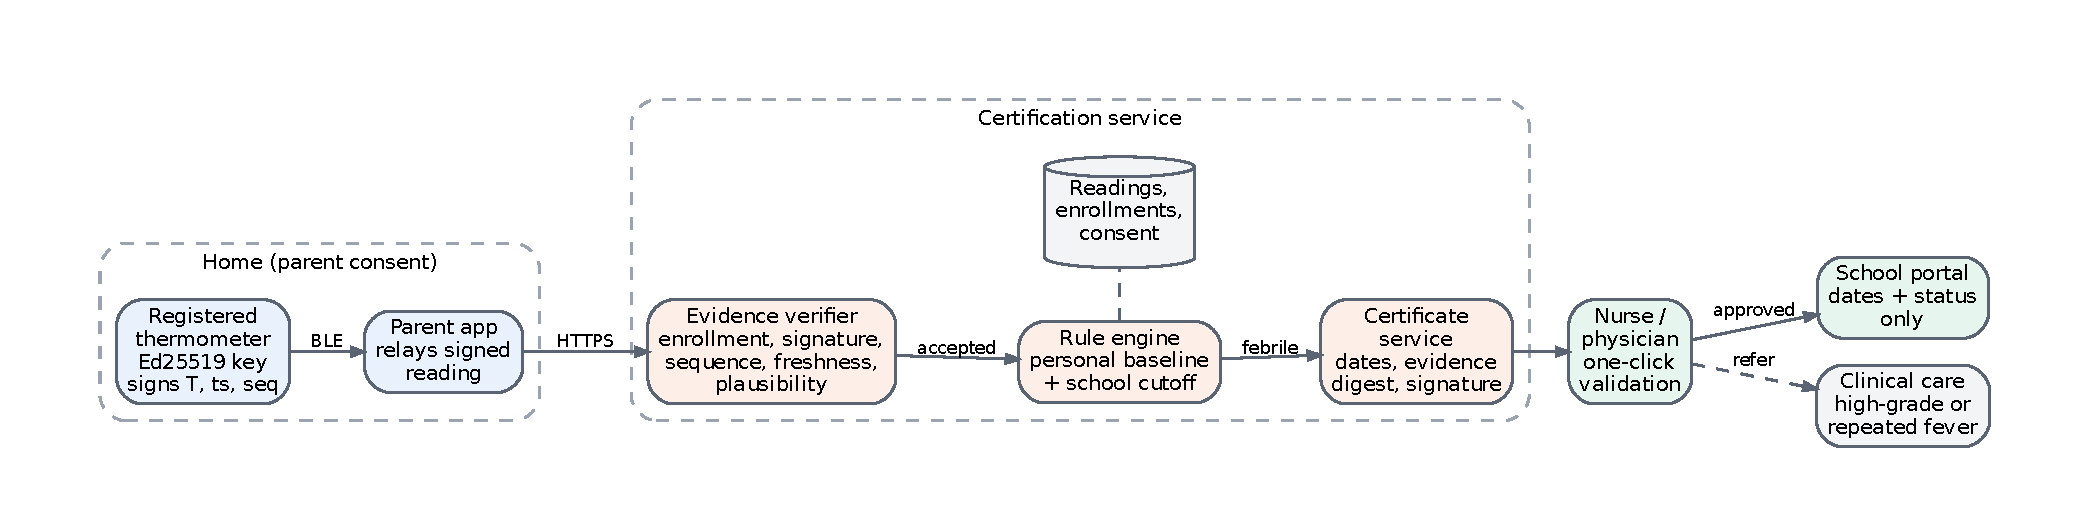
\includegraphics[width=\textwidth]{figures/architecture.pdf}
\caption{Architecture. The thermometer signs each reading; the service verifies it, applies the personal-baseline rule and issues a signed certificate that a nurse validates. The school portal receives dates and status only.}
\label{fig:arch}
\end{figure*}

\subsection{Registered Thermometer and Signed Reading}
At enrollment, with parental consent, the school registers a device ID and the device's Ed25519 public key \cite{rfc8032} against one student. The device holds the private key and never sees the student's identity. Each reading is a payload $\{\mathit{device\_id}, \mathit{seq}, \mathit{ts}, T, \mathit{site}, \mathit{nonce}\}$ encoded as canonical JSON and signed; a signed reading is \ReadingBytes{} bytes. In the proof of concept the thermometer is simulated in software; moving signing into firmware with a secure element is the path to hardware attestation.

\subsection{Evidence Verifier}
A reading is accepted only if: the device is enrolled and active; any claimed student matches the enrolled student; the signature verifies; $\mathit{seq}$ exceeds the last accepted value (anti-replay); $\mathit{ts}$ is not in the future (5\,min skew) and not older than 6\,h (freshness); and $34 \le T \le 43$\,\textdegree C (plausibility). Every rejection is logged with its reason.

\subsection{Personal-Baseline Rule}
The baseline $B$ is the median of the last 14 accepted readings below 37.5\,\textdegree C; with fewer than five such readings a population default of 36.8\,\textdegree C is used. A reading $T$ is febrile if
\begin{equation}
T \ge T_{\mathrm{fix}} \;\lor\; \left(T \ge T_{\mathrm{floor}} \land T - B \ge \Delta\right),
\label{eq:rule}
\end{equation}
with $T_{\mathrm{fix}} = 38.0$\,\textdegree C (the school policy, always honoured), $T_{\mathrm{floor}} = 37.5$\,\textdegree C and $\Delta = 1.0$\,\textdegree C. A febrile reading at or above 39.5\,\textdegree C, or on a third consecutive day, is escalated to clinical review instead of being certified. A deviation of at least 0.7\,\textdegree C without meeting (\ref{eq:rule}) is flagged as \emph{watch} with no certificate.

\begin{figure}[t]
\centering
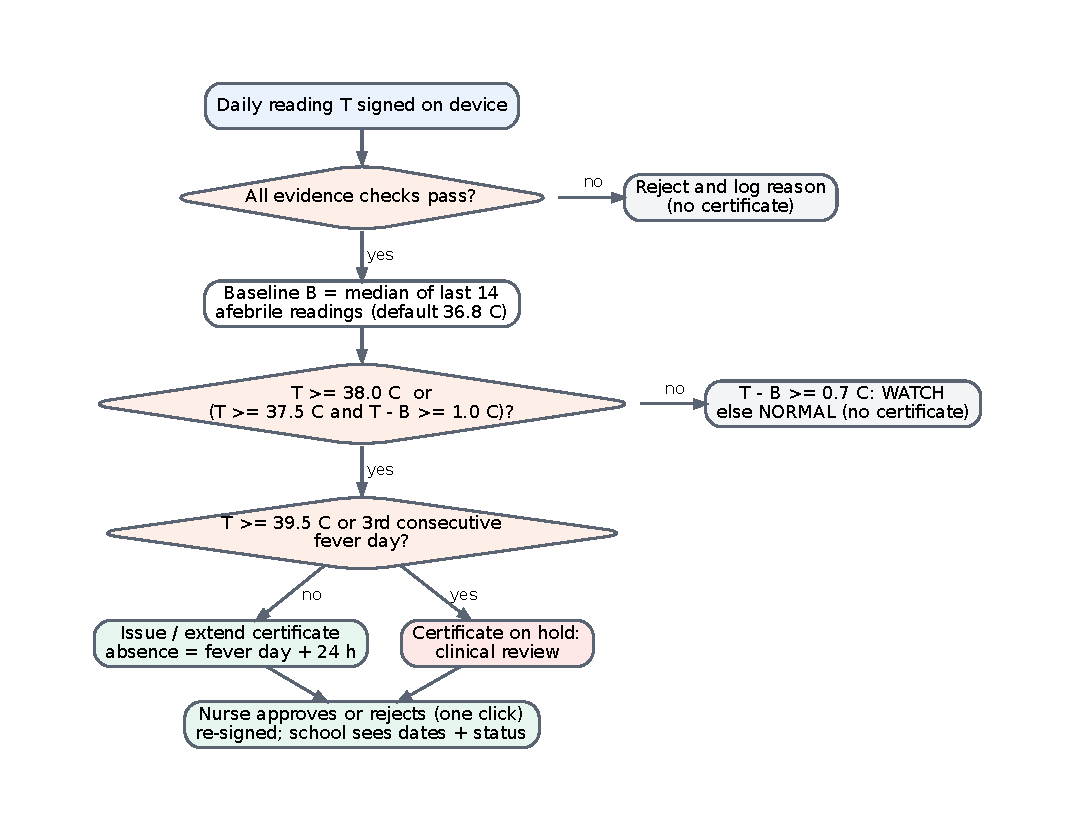
\includegraphics[width=0.92\columnwidth]{figures/flow.pdf}
\caption{Decision flow from a signed reading to a validated certificate.}
\label{fig:flow}
\end{figure}

\subsection{Certificate and Data Minimization}
A febrile reading creates or extends a certificate covering the fever day plus the 24\,h fever-free period. The certificate holds the certificate ID, student ID, absence dates, status, validator role and time, and a SHA-256 digest of the signed readings used as evidence; the service signs it and re-signs it on every change, so anyone with the issuer public key can verify it offline. Temperatures stay in the nurse console. The school portal shows only the reason (fever-related absence), the dates and the validation status, in line with the minimum-necessary principle for education records \cite{ferpa}.

\section{Evaluation}
\subsection{Detection on a Synthetic Cohort}
We simulated 500 students for 90 daily morning readings. Each student's normal temperature was drawn from $\mathcal{N}(36.7, 0.25^2)$\,\textdegree C, clipped to [36.0, 37.4], reflecting reported inter-individual differences \cite{obermeyer2017,diamond2021}. Readings added day-to-day variation ($\sigma = 0.15$\,\textdegree C), measurement noise ($\sigma = 0.10$\,\textdegree C) and 0.1\,\textdegree C display rounding. Fever episodes started with daily probability 0.012, lasted 1--3 days and raised temperature 1.0--2.5\,\textdegree C above the student's own normal; non-infectious transient rises of 0.3--0.8\,\textdegree C occurred on 3\% of other days. A day inside an episode was a fever day. After a 14-day warm-up, each seed gave about \FeverDays{} fever days in \Episodes{} episodes. The baseline was computed causally from past readings only.

\begin{table}[t]\centering\caption{Fever-day detection on the synthetic cohort (mean of 10 seeds; 38,000 student-days per seed after warm-up)}\label{tab:detection}\footnotesize\setlength{\tabcolsep}{3pt}
\begin{tabular}{lcccccc}\hline
Rule & Sens. & Sens.\,low & Spec. & PPV & F1 & FC \\\hline
Fixed 38.0\,\textdegree C & 0.810 & 0.648 & 0.9994 & 0.971 & 0.883 & 0.6 \\
Fixed 37.5\,\textdegree C & 0.975 & 0.931 & 0.9856 & 0.614 & 0.753 & 14.1 \\
Personal (ours) & 0.949 & 0.919 & 0.9987 & 0.943 & 0.946 & 1.3 \\
\hline\end{tabular}\\[2pt]\parbox{\columnwidth}{\scriptsize Sens.\,low: students in the lowest tertile of normal temperature. FC: false certificates per 1000 student-days.}\end{table}


Table~\ref{tab:detection} and Fig.~\ref{fig:results} summarize the results. The fixed 38.0\,\textdegree C rule missed many fever days in students with low normal temperatures. The personal-baseline rule recovered most of them, raising episode-level detection from \EpiFixed\% to \EpiPers\%, while adding less than one false certificate per 1000 student-days. Lowering the fixed cutoff to 37.5\,\textdegree C reached similar sensitivity, but it produced \FCLow{} false certificates per 1000 student-days, concentrated in students with high normal temperatures (specificity \SpecHighLow{} in that tertile). The personal rule had the highest F1 (\FOnePers{} vs \FOneFixed{} for the fixed 38.0\,\textdegree C rule). During the cold-start period, when the population default replaces the personal baseline, sensitivity was \ColdSensPers{}. Across nine combinations of inter-individual spread (0.15--0.35\,\textdegree C) and measurement noise (0.05--0.20\,\textdegree C), personal-rule sensitivity stayed at \SensRangePers{} (fixed 38.0\,\textdegree C: \SensRangeFixed{}), with \FCRangePers{} false certificates per 1000 student-days (fixed 37.5\,\textdegree C: \FCRangeLow{}).

\begin{figure}[t]
\centering
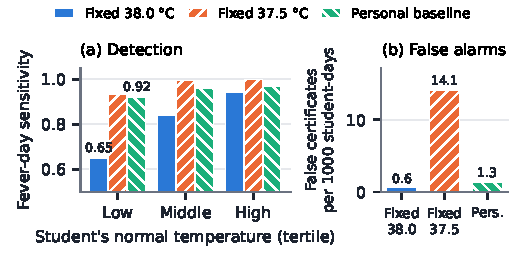
\includegraphics[width=\columnwidth]{figures/results.pdf}
\caption{(a) Fever-day sensitivity by tertile of students' normal temperature. (b) False certificates per 1000 student-days. Mean of \NSeeds{} seeds.}
\label{fig:results}
\end{figure}

\subsection{Tamper Evidence and Processing Time}
We enrolled 50 virtual thermometers, submitted 1000 genuine readings and ran 200 trials of each attack in Table~\ref{tab:tamper}. Every attack was rejected by the intended check, and every genuine reading was accepted. Altering any field of an issued certificate (dates, status or student) also failed signature verification in all 200 trials. On a commodity x86-64 machine (Python 3.13, single thread), median times were \SignMs{}\,ms to sign a reading, \VerifyMs{}\,ms to verify a signature, and \EtoEMs{}\,ms (95th percentile \EtoEPms{}\,ms) from receiving a reading to issuing a certificate. Approval by the nurse then completes the process, compared with a clinic visit to obtain a note.

\begin{table}[t]\centering\caption{Tamper-evidence tests (50 enrolled virtual thermometers)}\label{tab:tamper}\footnotesize\setlength{\tabcolsep}{3pt}
\begin{tabular}{p{4.1cm}p{2.0cm}r}\hline
Attack & Caught by & Detected \\\hline
Value edited after signing & signature & 200/200 \\
Timestamp back-dated after signing & signature & 200/200 \\
Replay of an accepted reading & sequence & 200/200 \\
Impersonation with a non-enrolled key & signature & 200/200 \\
Another student's device substituted & enrollment binding & 200/200 \\
Delayed (hoarded) genuine reading & freshness & 200/200 \\
Unregistered device & enrollment & 200/200 \\
Certificate field altered (dates, status, student) & issuer signature & 200/200 \\
\hline Genuine readings (accepted) & -- & 1000/1000 \\
\hline\end{tabular}\end{table}


\subsection{Bench Agreement (Protocol)}
Sensor accuracy is tested without human participants. The portable thermometer and a calibrated reference probe are held side by side in a stirred, temperature-controlled water bath at 36.0, 37.0, 37.5, 38.0, 39.0 and 40.0\,\textdegree C, with at least five paired readings per set point. Agreement is reported as Bland--Altman bias and 95\% limits of agreement \cite{bland1986}, together with agreement in classification at the 38.0\,\textdegree C cutoff. The analysis script is in the repository. \tbd{Results to be inserted after the bench test: n pairs, bias, limits of agreement, \% within $\pm$0.2\,\textdegree C, classification agreement.}

\section{Limitations}
The detection results come from a simulated cohort, and the gain depends on the assumed spread of normal temperatures and the noise. They should be confirmed with longitudinal readings from real students. Cryptographic checks prove that a reading came unaltered from an enrolled device. They cannot show that the probe was in the right child's mouth, or that it was not warmed. Nurse review, baseline-consistent fever dynamics and wearable sensing are partial mitigations. A reading taken after a fever-reducing medicine can mask a fever. The software key in the proof of concept must move into a secure element. The system documents a fever and does not diagnose its cause.

\section{Conclusion}
Treating a portable thermometer as a registered evidence device, and comparing its readings with the student's own baseline, turns a routine home measurement into a verifiable, privacy-preserving absence certificate. In simulation, the personal-baseline rule detected fevers that a fixed cutoff missed in students with low normal temperatures, without a matching rise in false certificates, and the evidence chain detected every scripted attack. Next steps are the bench test, firmware signing on a Bluetooth thermometer, and a pilot with school nurses.

\begin{thebibliography}{10}
\bibitem{cdc2024} Centers for Disease Control and Prevention, ``Respiratory virus guidance,'' Mar. 2024. [Online]. Available: \url{https://www.cdc.gov/respiratory-viruses/guidance/respiratory-virus-guidance.html}
\bibitem{miller2018} A.~C. Miller, I.~Singh, E.~Koehler, and P.~M. Polgreen, ``A smartphone-driven thermometer application for real-time population- and individual-level influenza surveillance,'' \emph{Clin. Infect. Dis.}, vol.~67, no.~3, pp.~388--397, 2018, doi: 10.1093/cid/ciy073.
\bibitem{chamberlain2020} S.~D. Chamberlain, I.~Singh, C.~Ariza, A.~Daitch, P.~Philips, and B.~D. Dalziel, ``Real-time detection of COVID-19 epicenters within the United States using a network of smart thermometers,'' medRxiv preprint, 2020, doi: 10.1101/2020.04.06.20039909.
\bibitem{besculides2005} M.~Besculides, R.~Heffernan, F.~Mostashari, and D.~Weiss, ``Evaluation of school absenteeism data for early outbreak detection, New York City,'' \emph{BMC Public Health}, vol.~5, art.~105, 2005, doi: 10.1186/1471-2458-5-105.
\bibitem{kara2011} E.~O. Kara \emph{et al.}, ``Absenteeism in schools during the 2009 influenza A(H1N1) pandemic: A useful tool for early detection of influenza activity in the community?'' \emph{Epidemiol. Infect.}, 2011, doi: 10.1017/S0950268811002093.
\bibitem{obermeyer2017} Z.~Obermeyer, J.~K. Samra, and S.~Mullainathan, ``Individual differences in normal body temperature: Longitudinal big data analysis of patient records,'' \emph{BMJ}, vol.~359, art.~j5468, 2017, doi: 10.1136/bmj.j5468.
\bibitem{diamond2021} A.~Diamond, C.~T. Lye, D.~Prasad, and D.~Abbott, ``One size does not fit all: Assuming the same normal body temperature for everyone is not justified,'' \emph{PLoS ONE}, vol.~16, no.~2, art.~e0245257, 2021, doi: 10.1371/journal.pone.0245257.
\bibitem{rfc8032} S.~Josefsson and I.~Liusvaara, ``Edwards-curve digital signature algorithm (EdDSA),'' IETF RFC 8032, Jan. 2017.
\bibitem{ferpa} Family Educational Rights and Privacy Act, 20 U.S.C. \S~1232g; 34 CFR Part 99.
\bibitem{bland1986} J.~M. Bland and D.~G. Altman, ``Statistical methods for assessing agreement between two methods of clinical measurement,'' \emph{Lancet}, vol.~1, no.~8476, pp.~307--310, 1986.
\end{thebibliography}
\end{document}
